\documentclass[10pt,a4paper,twoside]{article}
% The following LaTeX packages must be installed on your machine: amsmath, authblk, bm, booktabs, caption, dcolumn, fancyhdr, geometry, graphicx, hyperref, latexsym, natbib

% Please make sure that spp.dat (supplied with this template) is in your working directory or path
\input{spp.dat}
\usepackage{tabularray}
\usepackage{url}
\usepackage{xcolor}
\usepackage{soul}
\usepackage[belowskip=-15pt,aboveskip=0pt]{caption}
\definecolor{light-gray}{gray}{0.95}
\newcommand{\code}[1]{\colorbox{light-gray}{\texttt{#1}}}
%  Editorial staff will uncomment the next line
% \providecommand{\artnum}[0]{XX-XX}
% \renewcommand{\articlenum}[0]{SPP-\the\year-\artnum-}

\begin{document}

%--------------------------------------------------
%  Fill in the paper's title in the Sentence case
%  Titles beginning with articles (A, An, The) are discouraged
%--------------------------------------------------
\title{\TitleFont Fake News Detection in Philippine News Corpus using LDA and Sentiment Analysis with Machine Learning}
\vspace{-1.5em}
\author[*\negthickspace]{Renz Jamuel B. Jamen}
\author[ ]{Reinabelle C. Reyes\lastauthorsep}
\affil[ ]{National Institute of Physics, University of the Philippines, Diliman, Quezon City 1101, Philippines}
\affil[*]{\corremail{rjjamuel@nip.upd.edu.ph} }


\begin{abstract}
\noindent
%--------------------------------------------------
% Include abstract and keywords here
%--------------------------------------------------
The persistent proliferation of fake news on Philippine social media platforms poses serious threats to public discourse and safety. To address this growing concern, it is critical to continuously develop automated models that effectively classify online published news as either real or fake. This study presents an alternative approach to fake news classification by integrating VADER-extracted sentiment ratio and reduced feature vectors through Linear Discriminant Analysis (LDA) on a suite of supervised machine-learning models. We trained and evaluate these models on a publicly-available corpus of real and fake news from the Philippines. Remarkably, our best-performing model achieved an accuracy of 94\% using only a single feature derived from LDA applied to a combination of TF-IDF features and sentiment ratio, comparable to benchmark models in the literature. Moreover, the addition of the sentiment ratio consistently improved performance across models. Overall, this study provides valuable insights for improving fake news classifiers for Philippine-based news corpus.

\keywords{fake news, sentiment analysis, Linear Discriminant Analysis, supervised machine learning, Natural Language Processing}

\end{abstract}

\maketitle
\thispagestyle{titlestyle}


%--------------------------------------------------
% the main text of your paper begins here
%--------------------------------------------------
\section{Introduction}\label{sec:intro}
Fake news refers to stories disseminated through ostensible sources that intentionally misinform the public for various opportunistic purposes --not limited to influencing public opinion, weakening institutional trust, and exacerbating social and political tensions \cite{baptista}. The massive societal impacts brought by this persistent problem necessitate continuous research and development to combat them. Most performing solutions today involve machine learning and Natural Language Processing (NLP) techniques due to their speed, flexibility, and adaptability. At its core, fake news mimics real news formats. Their subtle differences in writing styles are leveraged by content-based detection models to determine news veracity \cite{janze_risius_2017, khanam}. This automated method, trained on a multitude of available text features, remains the simplest and most efficient as compared to the tedious process of fact-checking and information retrieval. Recent works also incorporate other features like sentiments \cite{ajao, Alonso}, as either the basis or complementary element, to effectively differentiate fake news from real news on international news corpora.

Fernandez and Devaraj have constructed a Philippine-based news corpus collected from online sources and developed fake news classification models trained on this  \cite{Fernandez}.   They did this by extracting linguistic-based cues (Word Count, Syllables Count, Articles\%, Prepositions\%, etc.) from both headlines and news content and identified the best feature set after fitting on supervised machine-learning models such as Gaussian Naïve Bayes (GNB), Logistic Regression (LR), and Support Vector Machines (SVM). In this work, we present an alternative approach using an efficient sentiment-aware technique to classify fake news articles from their dataset. We evaluate the impact of the addition of dimensionality reduction and sentiment ratio extracted using VADER (Valence Aware Dictionary for sEntiment Reasoning) on the model performance.

\section{Methodology}\label{sec:figures}
Figure \ref{fig:flow} illustrates the steps performed in this study, namely pre-processing, feature engineering, modeling, and evaluation. Each step is detailed in the following subsections.
\begin{figure}[h!]
    \centering
    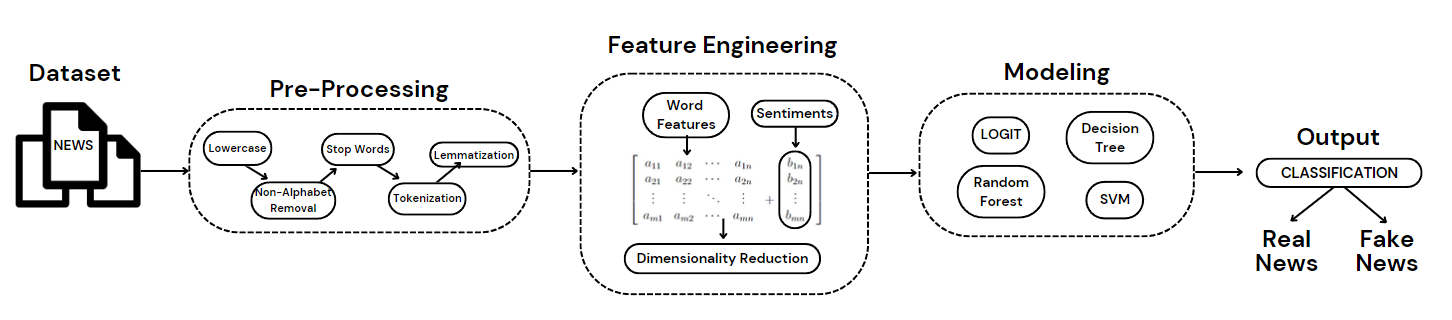
\includegraphics[width=\textwidth]{Figures/flow_bw.png}
    \caption{Flowchart illustrating development of machine learning models for Fake News classification}
    \captionsetup{belowskip=0pt}
    \label{fig:flow}
\end{figure}\vspace{-0.5em}

\subsection{Dataset} 
We utilized the publicly-available Philippine Fake News corpus compiled by Aaron Carl Fernandez from Mapua Institute of Technology, Philippines \cite{Fernandez}. The corpus consists of 22,458 local articles in English from January 1, 2016 to October 31, 2018. Credible news samples were obtained from the three national broadsheets: The Philippine Daily Inquirer, Manila Bulletin, and The Manila Times. Non-credible samples were extracted from fake news websites identified by the Philippine Senate, Center for Media Freedom and Responsibility, and Catholic Bishop's Conference in the Philippines. All news samples from both classes belong to the ``Nation" news category, ensuring consistency in news genre and article length.
\vspace{-1.7em}
\subsection{Pre-processing} 
The text data underwent a series of cleaning processes using the Texthero python package \cite{Besomi_2023}. Using the {\color{gray}\texttt{clean}} function, all strings were turned into lowercase and all non-alphabet characters were removed. We omitted all words less than three characters and stop-words (such as ``the", ``and", ``is", etc.).  The cleaned words were tokenized and finally turned into lemmas or base forms using {\color{gray}\texttt{WordNetLemmatizer}}  of the Natural Language Tool Kit. After cleaning, we randomly sampled a balanced number of articles, shuffled, and split them into training and testing sets using a 70:30 ratio. Our final dataset contains 7,625 Real News and 7,100 Fake News samples, comprising 52\% and 48\% of the full dataset, respectively. 
\vspace{-0.5em}
\subsection{Feature Engineering} 
Word features were represented as unigrams using the term frequency-inverse document frequency (TF-IDF) method of the Scikit-learn library. It is an occurrence-based vectorizer that accounts for the weights of word tokens. The weights are the product of the two terms: TF (frequency of word $w$ in a document normalized by dividing it by the total number of words inside the document)  and IDF (log of the ratio between the total number of documents over the number of documents with the word $w$). We considered the top 10,000 word features and then applied filtering methods such that constant features (features containing only one value for all outputs in the dataset) were dropped. This resulted in a reduction to  1035 relevant features, which served as our baseline set of features.

To test whether fake news classification will be improved by the addition of sentiment scores, we calculate these scores using the lexicon-based scorer, VADER which analyzes text and assigns summed negative, neutral, and positive valence scores for each news article ranging from 0 to 1 \cite{VADER}. Each article was assigned a sentiment ratio, which we defined as the sum of the negative and positive scores divided by the sum of the neutral scores in each article. To examine the relationship between the sentiment ratio and our target news labels, we employed the point-biserial correlation, which specifically measures the association between a continuous variable (sentiment ratio) and a binary variable (Real or Fake News labels).  We find that the sentiment ratio and our target news labels are weakly positively correlated with a point-biserial correlation coefficient of $r$ = 0.17 and a significant p-value of $p < 0.001$.

We employ Linear Discriminant Analysis (LDA) to reduce the high feature vector dimension to a single feature, equal to one (1) less than the number of classes. LDA computes linear combinations of the features to generate two scatter matrices. Minimizing the within-class scatter matrix allows news samples from the same class to be grouped as closely as possible. Simultaneously, maximizing the between-class scatter matrix separates samples from different classes as far as possible. Through this technique, the features are projected into a new 1D axis that shows the effective separation of news classes.

We compare the performance of models using different features namely: (1) word features using TF-IDF (baseline), (2) TF-IDF and sentiment ratio, (3) LDA feature from TF-IDF, and (4) LDA feature from the combination of TF-IDF and sentiment ratio.
\vspace{-0.5em}
\subsection{Machine Learning Models and Performance Measures}
We selected the four simple and most commonly-used supervised machine-learning models: Logistic Regression (LR), Support Vector Machines (SVM), Decision Tree (DT), and Random Forest (RF) to facilitate faster computation and easier interpretability while also ensuring straightforward replication of our study. To train and evaluate these models, we performed five-fold cross-validation using {\color{gray}\texttt{GridSearchCV}} on the training set. This involved training the models on four training folds and evaluating them on the validation fold with the following set of hyperparameters: regularization parameter C (0.01, 0.1, 1, 10, 100) for LR and SVM, the maximum depth (2, 4, 6, 8, 10) for DT, and the number of trees (100, 200, 300, 400, 500) for RF. The process was repeated for all values in the grid and the optimal values for each model (reported in Table 1) with the highest cross-validation accuracy were selected.

After this, the models are evaluated on the independent testing set for an unbiased estimate of model performance. To each, we feed the four combinations of input features described above, generating a total of 16 trained models. We used accuracy, precision, recall, and F1-score, to assess the models' performance and compare them with those reported in the literature as these four are the widely accepted metrics for evaluating binary classification models.



\vspace{-0.8em}
\section{Results and Discussion}
The performance metrics of the developed models are summarized in Table \ref{results1}. We find that the SVM model consistently achieved the highest or second-highest test accuracy across all features, with the LDA feature from TF-IDF and sentiment ratio achieving the highest test accuracy of 93.78\%. This result is on par with the best-performing model in \cite{Fernandez} having an accuracy of 94.42\%  utilizing linguistic-based features extracted from both headlines and news contents using SVM.
\vspace{10pt}
\begin{table}[h!]
\centering
\caption{Performance metrics of models using different feature combinations from the PH Fake News dataset. The highest performance metric among the models for each feature combination is shown in bold.}
\label{results1}
\resizebox{\linewidth}{!}{
\begin{tblr}{
  row{2} = {c},
  column{3} = {c},
  cell{1}{1} = {r=2}{c},
  cell{1}{2} = {r=2}{c},
  cell{1}{3} = {r=2}{},
  cell{1}{4} = {r=2}{c},
  cell{1}{5} = {r=2}{c},
  cell{1}{7} = {c=4}{c},
  cell{3}{2} = {r=4}{},
  cell{3}{3} = {r=4}{},
  cell{3}{6} = {c},
  cell{3}{7} = {c},
  cell{3}{8} = {c},
  cell{3}{9} = {c},
  cell{3}{10} = {c},
  cell{4}{6} = {c},
  cell{4}{7} = {c},
  cell{4}{8} = {c},
  cell{4}{9} = {c},
  cell{4}{10} = {c},
  cell{5}{6} = {c},
  cell{5}{7} = {c},
  cell{5}{8} = {c},
  cell{5}{9} = {c},
  cell{5}{10} = {c},
  cell{6}{6} = {c},
  cell{6}{7} = {c},
  cell{6}{8} = {c},
  cell{6}{9} = {c},
  cell{6}{10} = {c},
  cell{7}{6} = {c},
  cell{7}{7} = {c},
  cell{7}{8} = {c},
  cell{7}{9} = {c},
  cell{7}{10} = {c},
  cell{8}{2} = {r=4}{},
  cell{8}{3} = {r=4}{},
  cell{8}{6} = {c},
  cell{8}{7} = {c},
  cell{8}{8} = {c},
  cell{8}{9} = {c},
  cell{8}{10} = {c},
  cell{9}{6} = {c},
  cell{9}{7} = {c},
  cell{9}{8} = {c},
  cell{9}{9} = {c},
  cell{9}{10} = {c},
  cell{10}{6} = {c},
  cell{10}{7} = {c},
  cell{10}{8} = {c},
  cell{10}{9} = {c},
  cell{10}{10} = {c},
  cell{11}{6} = {c},
  cell{11}{7} = {c},
  cell{11}{8} = {c},
  cell{11}{9} = {c},
  cell{11}{10} = {c},
  cell{12}{6} = {c},
  cell{12}{7} = {c},
  cell{12}{8} = {c},
  cell{12}{9} = {c},
  cell{12}{10} = {c},
  cell{13}{2} = {r=4}{},
  cell{13}{3} = {r=4}{},
  cell{13}{6} = {c},
  cell{13}{7} = {c},
  cell{13}{8} = {c},
  cell{13}{9} = {c},
  cell{13}{10} = {c},
  cell{14}{6} = {c},
  cell{14}{7} = {c},
  cell{14}{8} = {c},
  cell{14}{9} = {c},
  cell{14}{10} = {c},
  cell{15}{6} = {c},
  cell{15}{7} = {c},
  cell{15}{8} = {c},
  cell{15}{9} = {c},
  cell{15}{10} = {c},
  cell{16}{6} = {c},
  cell{16}{7} = {c},
  cell{16}{8} = {c},
  cell{16}{9} = {c},
  cell{16}{10} = {c},
  cell{17}{6} = {c},
  cell{17}{7} = {c},
  cell{17}{8} = {c},
  cell{17}{9} = {c},
  cell{17}{10} = {c},
  cell{18}{2} = {r=4}{},
  cell{18}{3} = {r=4}{},
  cell{18}{6} = {c},
  cell{18}{7} = {c},
  cell{18}{8} = {c},
  cell{18}{9} = {c},
  cell{18}{10} = {c},
  cell{19}{6} = {c},
  cell{19}{7} = {c},
  cell{19}{8} = {c},
  cell{19}{9} = {c},
  cell{19}{10} = {c},
  cell{20}{6} = {c},
  cell{20}{7} = {c},
  cell{20}{8} = {c},
  cell{20}{9} = {c},
  cell{20}{10} = {c},
  cell{21}{6} = {c},
  cell{21}{7} = {c},
  cell{21}{8} = {c},
  cell{21}{9} = {c},
  cell{21}{10} = {c},
  hline{1,3,22} = {-}{},
  hline{2} = {7-10}{},
}
~Model & ~Features                                                  & { No. of \\Features} & Hyperparameters     & {Cross-validation\\Accuracy} &  & Test Set       &                &                &                 \\
       &                                                            &                      &                     &                &  & Accuracy       & Precision      & Recall         & F1-score        \\
LR     & {TF-IDF\\(Baseline)}                                       & 1035                 & C = 1~ ~            & 87.343 (\pm\; 0.003)  &  & 87.72          & \textbf{85.88} & 86.93          & 86.40           \\
SVM    &                                                            &                      & C = 0.1             & 88.528 (\pm\; 0.003)  &  & \textbf{87.87} & 85.48          & \textbf{87.89} & \textbf{86.67 } \\
DT     &                                                            &                      & max\_depth = 10     & 77.544 (\pm\;0.008)  &  & 77.22          & 75.07          & 73.71          & 74.38           \\
RF     &                                                            &                      & n\_estimators = 500 & 87.948 (\pm\;0.004)  &  & 87.77          & 85.78          & 87.20          & 86.49           \\
       &                                                            &                      &                     &                &  &                &                &                &                 \\
LR     & {TF-IDF +\\sentiment \\ratio}                              & 1036                 & C = 1~ ~            & 88.523 (\pm\;0.006)  &  & 87.84          & 86.15          & 86.88          & 86.51           \\
SVM    &                                                            &                      & C = 0.1             & 88.409 (\pm\;0.003)  &  & \textbf{87.89} & 85.49          & \textbf{87.95} & 86.70           \\
DT     &                                                            &                      & max\_depth = 10     & 78.027 (\pm\;0.011)  &  & 77.44          & 74.95          & 74.67          & 74.81           \\
RF     &                                                            &                      & n\_estimators = 500 & 88.402 (\pm\;0.005)  &  & 88.18          & \textbf{86.25} & 87.63          & \textbf{86.93}  \\
       &                                                            &                      &                     &                &  &                &                &                &                 \\
LR     & {LDA feature \\(applied to \\TF-IDF)}                      & 1                    & C = 0.1~ ~          & 93.308 (\pm\;0.005)  &  & \textbf{93.40} & \textbf{92.19} & 93.17          & 92.68           \\
SVM    &                                                            &                      & C = 1               & 93.835 (\pm\;0.007)  &  & 93.35          & 91.05          & \textbf{94.45} & \textbf{92.72}  \\
DT     &                                                            &                      & max\_depth = 2      & 88.641 (\pm\;0.006)  &  & 88.20          & 87.03          & 86.61          & 86.82           \\
RF     &                                                            &                      & n\_estimators = 100 & 88.685 (\pm\;0.006)  &  & 88.20          & 87.03          & 86.61          & 86.82           \\
       &                                                            &                      &                     &                &  &                &                &                &                 \\
LR     & {LDA feature\\ (applied to \\TF-IDF+ \\sentiment \\ratio)} & 1                    & C = 0.1~ ~          & 93.649 (\pm\;0.006)  &  & 93.49          & \textbf{92.30} & 93.28          & 92.79           \\
SVM    &                                                            &                      & C = 1               & 94.171 (\pm\;0.007)  &  & \textbf{93.78} & 91.77          & \textbf{94.61} & \textbf{93.17 } \\
DT     &                                                            &                      & max\_depth = 2      & 88.782 (\pm\;0.006)  &  & 88.42          & 87.41          & 86.67          & 87.04           \\
RF     &                                                            &                      & n\_estimators = 100 & 88.936 (\pm\;0.005)  &  & 88.44          & 87.46          & 86.67          & 87.06           
\end{tblr}}
\end{table}
\vspace{-0.5em}

Using a single LDA feature led to significant improvements in model performance, as seen in Table 1 and from the SVM model's confusion matrices presented in Figure \ref{fig:conf}.  Specifically, there is a significant reduction in false positives from 13.6\% to 8.3\% and in false negatives from  8.7\% to 4.5\%  after applying LDA to both TF-IDF and sentiment ratio (Figure \ref{fig:conf}d with Figure \ref{fig:conf}b). These results align with enhanced precision and recall. Furthermore, Figure \ref{fig:example}a illustrates the discriminative power of LDA in effectively separating Real and Fake News articles within the test dataset, with well-separated Gaussian curves and distinct means, ultimately contributing to a significant performance boost for the models. 

We also find that incorporating the sentiment ratio resulted in a small but consistent performance boost across all models. Figure \ref{fig:example}b shows the distribution of the sentiment ratio for both classes. The sentiment ratio distribution for Fake News articles is skewed right with a slightly higher mean of 0.133 as compared to Real News with a mean of 0.108. We also observe a small percentage of Fake News articles with a high sentiment ratio. This valuable information augments the predictive capabilities of our models, contributing to their improved performance.

Quantitatively, the relative importance of the LDA and sentiment ratio in the DT and RF models, as measured by the mean decrease in impurity (MDI) are 0.86 and 0.16, respectively.

Finally, it is worth highlighting the remarkable decrease in training run times achieved through feature reduction using LDA. As a measure of real-time performance, we used the wall time measured by the time function in Python. The results demonstrate efficiency in the run time of the SVM model with a 94\% reduction from 30.5 s to 1.87 s.

\vspace{-1em}
\begin{figure}[h!]
    \centering
    \subfloat[TF-IDF]{{\includegraphics[width=2.9cm]{Figures/svm_1.png} }}%
    \subfloat[TF-IDF + SR]{{\includegraphics[width=3.2cm]{Figures/svm_2.png} }}%
     \subfloat[LDA (TF-IDF)]{{\includegraphics[width=3.2cm]{Figures/svm_3.png} }}%
     \subfloat[LDA (TF-IDF + SR)]{{\includegraphics[width=3.6cm]{Figures/svm_4.png} }}%
    \caption{Confusion matrices for the testing set using different feature combinations with the SVM model}%
    \label{fig:conf}%
\end{figure}

\begin{figure}[h!]
    \centering
    \subfloat{{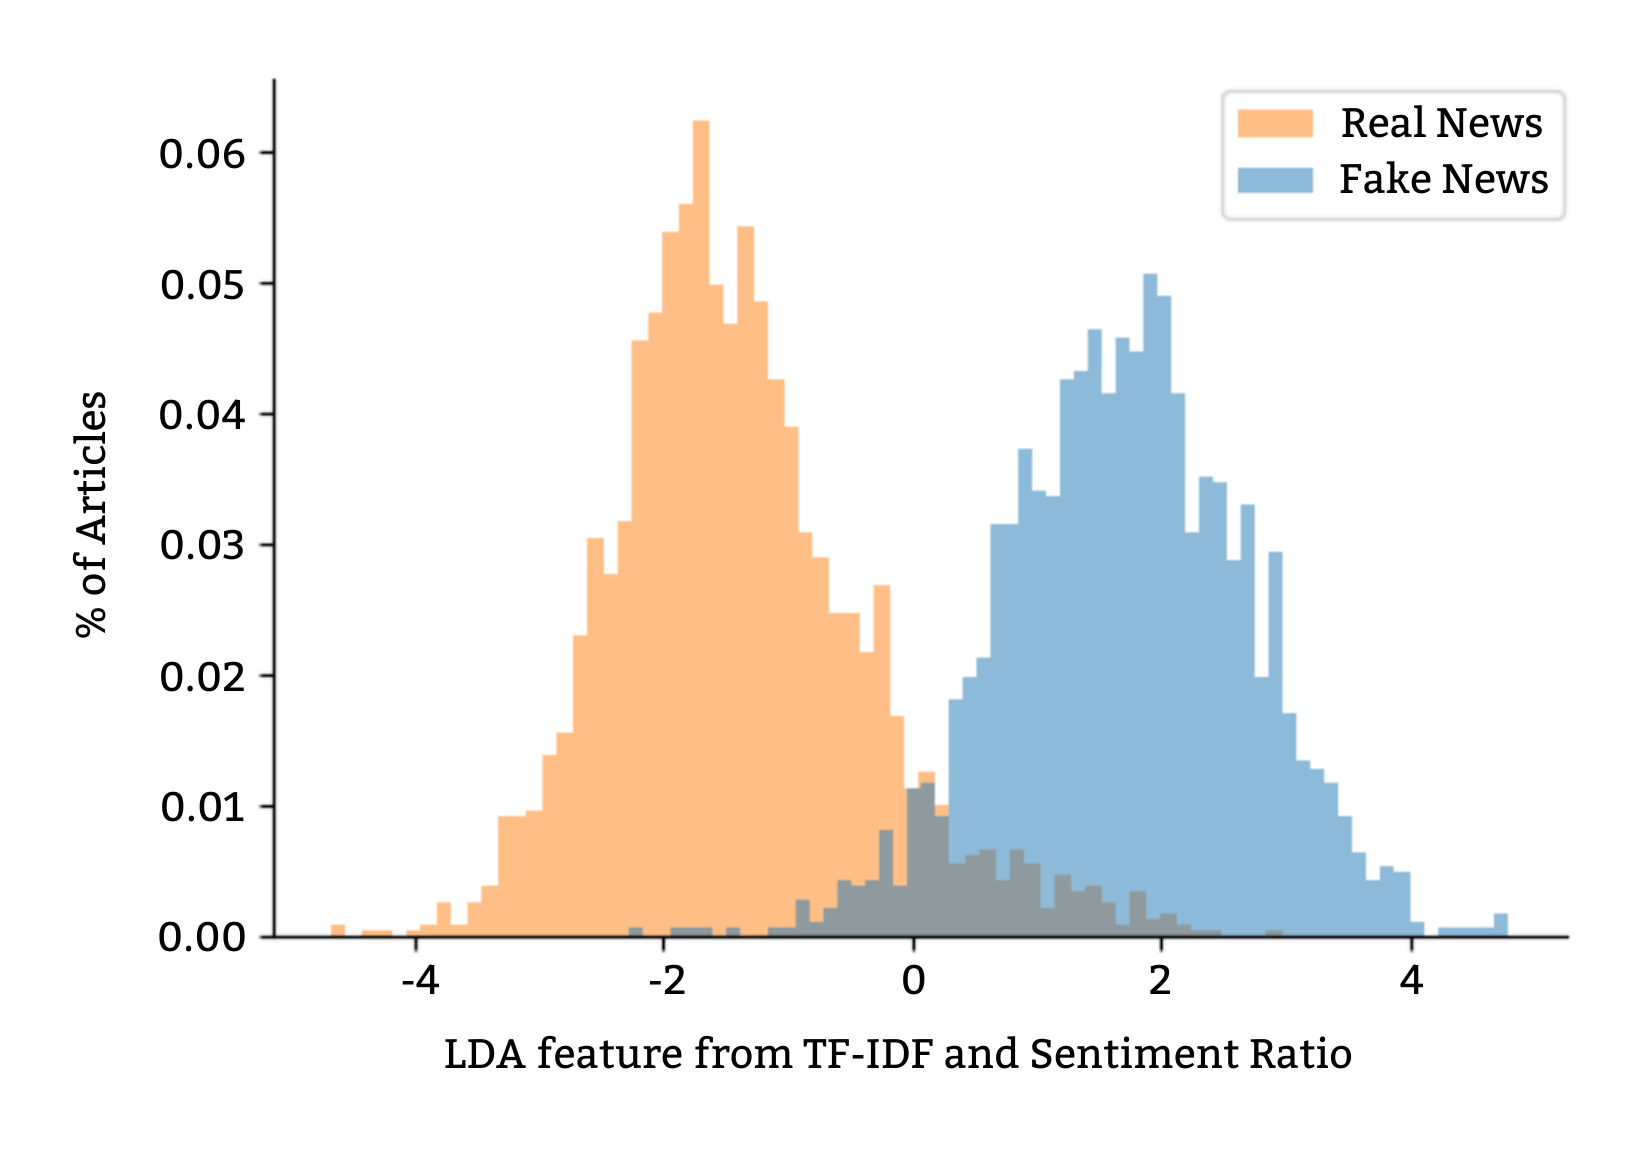
\includegraphics[width=6cm]{Figures/new_1.png} }}%
    \qquad
    \subfloat{{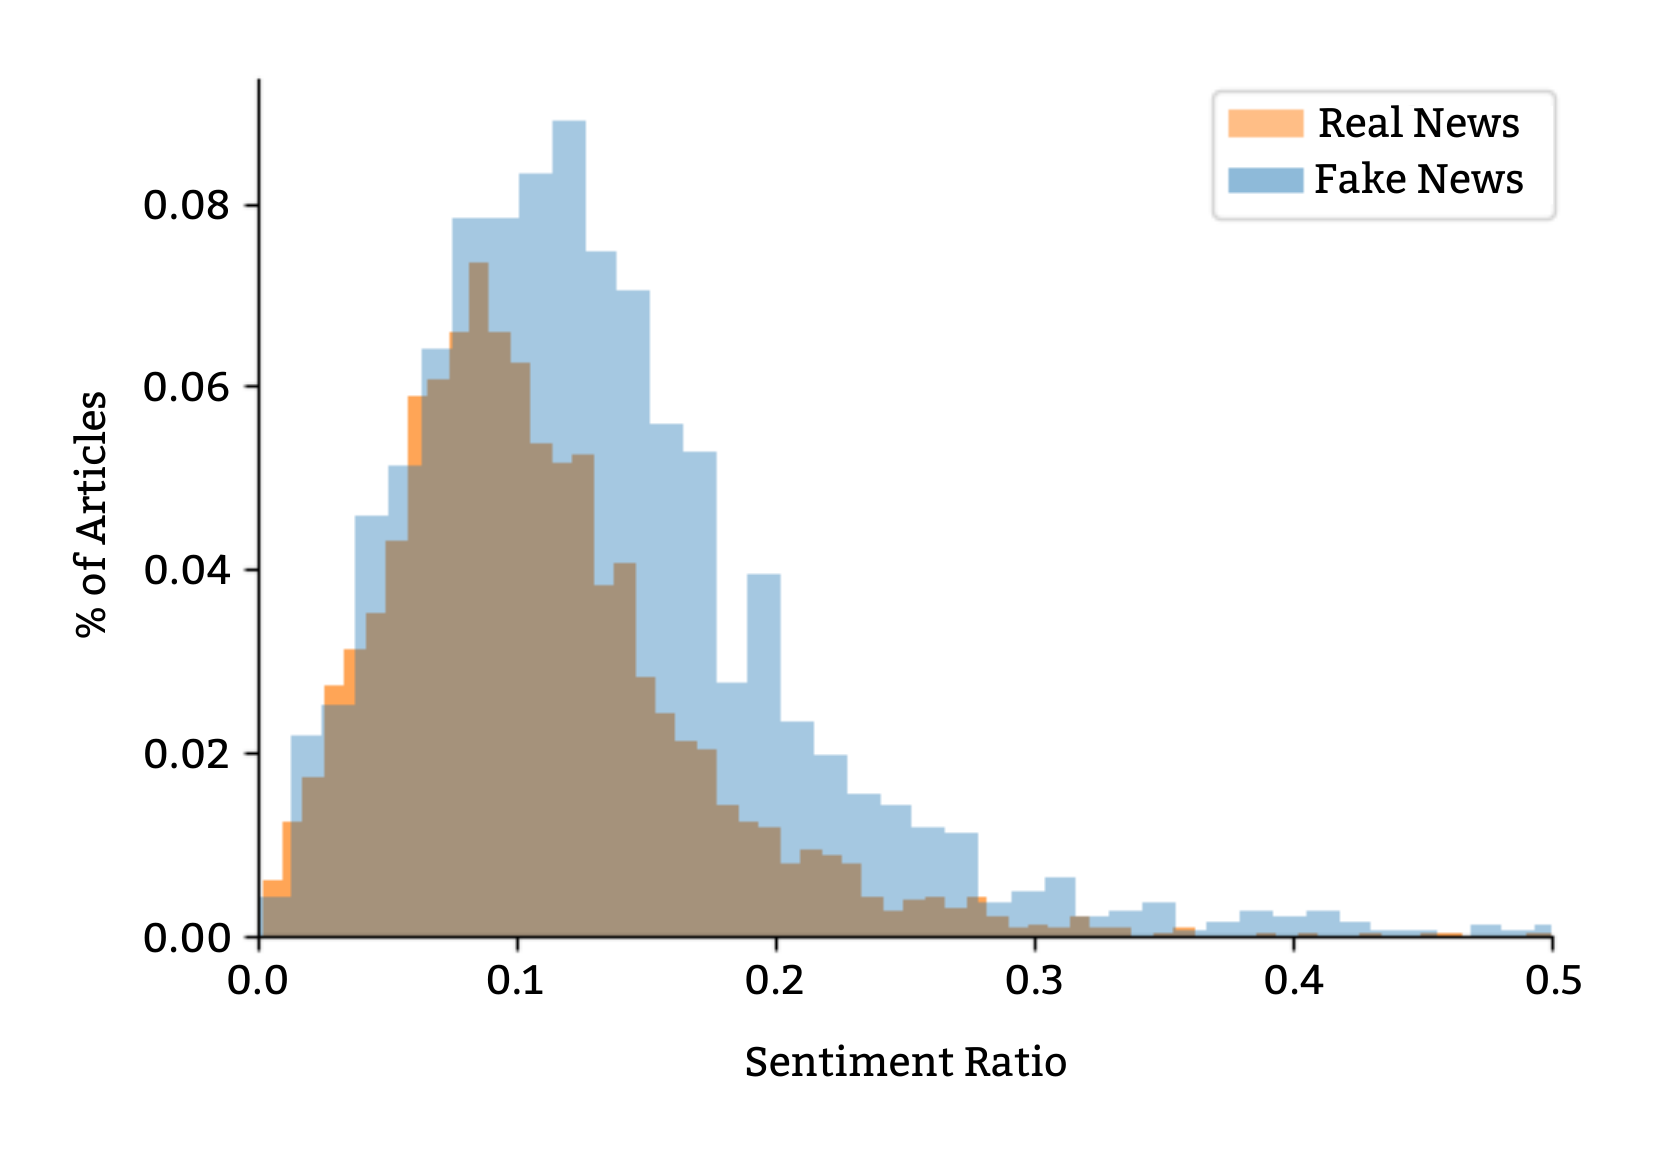
\includegraphics[width=6cm]{Figures/new_2.png} }}%
    \caption{Histograms showing class separability between Real and Fake News  through the (a) LDA feature from TF-IDF and sentiment ratio combined and (b) sentiment ratio}%
    \label{fig:example}%
\end{figure}

\section{Conclusions and Future Work}
In this study, we leveraged LDA and sentiment analysis as additional feature engineering techniques for supervised machine-learning models to effectively classify Philippine-based online news articles as either real or fake. Remarkably, our final model, using only one reduced feature, achieved accuracy significantly higher than the baseline model that relied on thousands of features, and on par with an existing model relying on linguistic-based cues derived from the text \cite{Fernandez}. 

 In further work, we aim to apply this method to other publicly-available international fake news corpora for comparison. We will also explore alternative dimensionality reduction techniques and sentiment scorers to expand the analysis and overcome the limitations associated with relying exclusively on LDA and VADER.  Furthermore, we will conduct a more thorough error analysis on the models to gain insights into the specific types of misclassifications and identify areas where the machine learning models struggled in classifying news articles accurately. Exploring these false positive and false negative cases opens potential avenues for improvement. These efforts will not only refine the existing models but also enhance our understanding of fake news detection within the Philippine context.\vspace{-0.5em}

\bibliographystyle{spp-bst}
\bibliography{bibfile}

\end{document}